% ---
% Capa
% ---
\imprimircapa
% ---

% ---
% Folha de rosto
% (o * indica que haverá a ficha bibliográfica)
% ---
\imprimirfolhaderosto*
% ---

% ---
% Inserir a ficha bibliografica
% ---
% http://ficha.bu.ufsc.br/
\begin{fichacatalografica}
	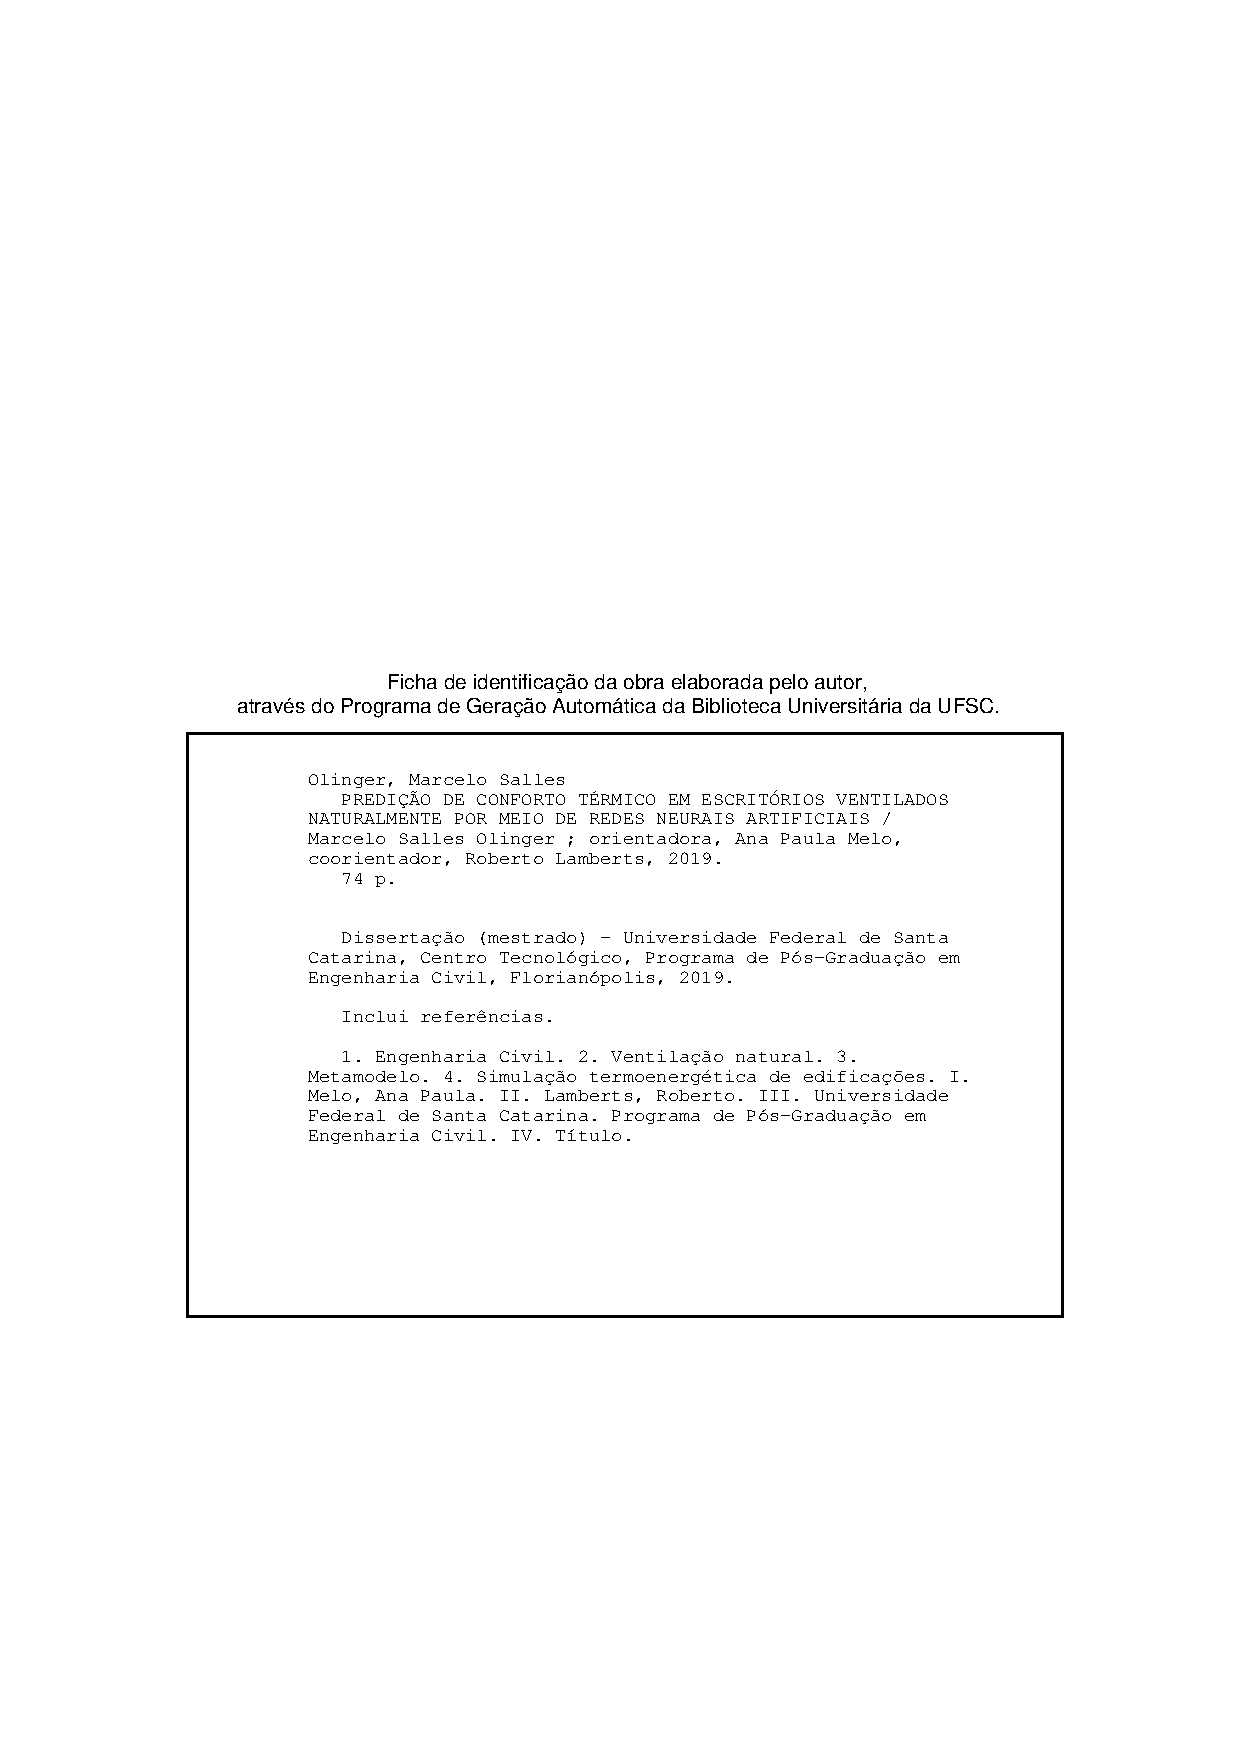
\includepdf{beforetext/Ficha_Catalografica.pdf}
\end{fichacatalografica}
% ---

% ---
% Inserir folha de aprovação
% ---
\begin{folhadeaprovacao}
	\OnehalfSpacing
	\centering
	\imprimirautor\\%
	\vspace*{10pt}		
	\textbf{\imprimirtitulo}%
	\ifnotempty{\imprimirsubtitulo}{:~\imprimirsubtitulo}\\%
	%		\vspace*{31.5pt}%3\baselineskip
	\vspace*{\baselineskip}
	%\begin{minipage}{\textwidth}
	O presente trabalho em nível de \imprimirnivel~foi avaliado e aprovado por banca examinadora composta pelos seguintes membros:\\
	%\end{minipage}%
	\vspace*{\baselineskip}
	Prof. Saulo Güths, Dr.\\
	Universidade Federal de Santa Catarina\\
	\vspace*{\baselineskip}
	Prof. Martin Gabriel Ordenes Mizgier, Dr.\\
	Universidade Federal de Santa Catarina\\
	\vspace*{\baselineskip}
	Facundo Bre, Dr.\\
	Universidad Nacional del Litoral, Argentina\\
	\vspace*{2\baselineskip}
	\begin{minipage}{\textwidth}
		Certificamos que esta é a \textbf{versão original e final} do trabalho de conclusão que foi julgado adequado para obtenção do título de \imprimirformacao.\\
	\end{minipage}
	%    \vspace{-0.7cm}
	\vspace*{\fill}
	\assinatura{\OnehalfSpacing\imprimircoordenador \\ \imprimircoordenadorRotulo~do Programa}
	\vspace*{\fill}
	\assinatura{\OnehalfSpacing\imprimirorientador \\ \imprimirorientadorRotulo}
	%	\ifnotempty{\imprimircoorientador}{
	%	\assinatura{\imprimircoorientador \\ \imprimircoorientadorRotulo \\
	%		\imprimirinstituicao~--~\imprimirinstituicaosigla}
	%	}
	% \newpage
	\vspace*{\fill}
	\imprimirlocal, \imprimirdata.
\end{folhadeaprovacao}
% ---

% ---
% Dedicatória
% ---
%\begin{dedicatoria}
%	\vspace*{\fill}
%	\noindent
%	\begin{adjustwidth*}{}{5.5cm}     
%		Este trabalho é dedicado aos meus colegas de classe e aos meus queridos pais.
%	\end{adjustwidth*}
%\end{dedicatoria}
% ---

% ---
% Agradecimentos
% ---
\begin{agradecimentos}
	Agradeço, primeiramente, à minha família.
	Minhas conquistas de hoje são o resultado de ações que começaram muito antes da minha existência, e os valores que tenho vêm sendo passado desde meus bisavós e avós, até aos meus pais.
	Aos meus irmãos, tios e primos, que convivem comigo desde sempre, e são pessoas com quem eu sei que posso sempre contar.
	À minha noiva, Camila, que me acompanhou durante todo o mestrado e que estará sempre ao meu lado para os próximos desafios.
	
	Agradeço aos meus professores. Àqueles que contribuíram para minha formação desde a base, até às disciplinas de pós-graduação. 
	À Profa. Letícia Neves, que disponibilizou o banco de dados utilizado neste estudo e que esteve presente como membro da banca na minha qualificação.
	Aos professores da banca examinadora, Saulo Güths, Martin Mizgier e Facundo Bre, pelas suas contribuições ao trabalho.
	Aos meus orientadores, Ana Paula Melo e Roberto Lamberts, por todo aprendizado que vai muito além da eficiência energética em edificações.
	
	Agradeço aos meus colegas do LabEEE. Formamos uma excelente equipe, com grande potencial, e muito divertida.
	Ao Leonardo Mazzaferro, por me apresentar o mundo da eficiência energética em edificações, e pela parceria forte ao longo de todos esses anos.
	
	Aos auxílios financeiros da CNPq e CAPES, e à infraestrutura disponibilizada pela UFSC.
	
	Finalmente, agradeço a todos os meus amigos, e aqueles que de alguma forma contribuíram e contribuem para o meu crescimento como acadêmico e como pessoa.
	
	Obrigado!
\end{agradecimentos}
% ---

% ---
% Epígrafe
% ---
\begin{epigrafe}
	\vspace*{\fill}
	\begin{flushright}
		\textit{``All models are wrong, but some are useful.''\\
			(George E. P. Box)}
	\end{flushright}
\end{epigrafe}
% ---

% ---
% RESUMOS
% ---

% resumo em português
\setlength{\absparsep}{18pt} % ajusta o espaçamento dos parágrafos do resumo
\begin{resumo}
	\SingleSpacing
	O condicionamento de ar para resfriamento de edificações é responsável por parcela significativa do consumo energético no mundo, e isso tende a aumentar nas próximas décadas. Uma solução para a mitigação do aumento no consumo de energia para resfriamento de ar é uso de ventilação natural (VN). 
	A VN é uma técnica de resfiramento passivo com um potencial significativo de aplicação em países de clima quente. 
	Apesar de seu pontencial de aplicabilidade, o uso de VN em edifícios de escritórios
	vem diminuindo gradualmente no Brasil, pois edificações de escritórios recentes vêm sendo projetadas exclusivamente com sistemas de condicionamento de ar.	
	Para que seja aplicada de forma efetiva, é importante que a VN seja concebida desde a fase inicial de projeto. Durante a fase inicial de projeto, há pouco detalhamento relacionado ao projeto arquitetônico, e há necessidade de agilidade nas tomadas de decisão.
	Diante deste cenário, uma ferramenta capaz de estimar o conforto térmico em edificações de forma simples e rápida pode ser de grande utilidade.	
	O objetivo deste estudo é desenvolver um metamodelo de rede neural artificial capaz de estimar o conforto térmico em edificações de escritórios ventilados naturalmente. 
	O indicador de conforto térmico utilizado é a fração de horas do ano em que há desconforto térmico por calor no ambiente (EHF), de acordo com o método adaptativo da ASHRAE Standard 55 (2017), para 80\% de aceitabilidade entre os ocupantes.	
	O metamodelo é desenvolvido a partir de uma base de dados de simulações termoenergéticas obtidas através do programa computacional EnergyPlus. Os modelos que compõem a base de dados foram definidos a partir das características comumente encontradas em edificações de escritórios da cidade de São Paulo. A definição dos parâmetros variados no desenvolvimento dos modelos é estabelecida através da análise de sensibilidade global de Sobol.	
	O treinamento da rede neural artificial é realizado com uma base de dados de 100.000 simulações termoenergéticas, amostradas pelo método de amostragem do hipercubo latino. 
	O desempenho do metamodelo foi avaliado para uma amostra de validação com 20.000 casos, e obteve resultados de EHF com um erro absoluto médio igual a 0,009, e um erro absoluto do 95º percentil igual a 0,024.	
	O metamodelo desenvolvido foi capaz de estimar o conforto térmico em edificações de escritórios ventilados naturalmente para a cidade de São Paulo com resultados próximos aos obtidos pelo programa de simulação computacional EnergyPlus.
	Esse metamodelo pode ser utilizado por projetistas como uma ferramenta de fácil aplicação no suporte à tomada de decisão em fases iniciais de projeto.
	
	\textbf{Palavras-chave}: Ventilação natural. Metamodelo. Simulação termoenergética de edificações.
\end{resumo}

% resumo em inglês
\begin{resumo}[Abstract]
	\SingleSpacing
	\begin{otherlanguage*}{english}
		Energy demand in the world for air cooling in buildings is significant, and it is expected to increase in the next decades.
		Natural ventilation (NV) could be a solution to mitigate energy use for air cooling, since it is a passive cooling strategy with significant potential for hot climates.
		Despite its potential, the use of NV has been decreasing in recent years for office buildings in Brazil, since the design of buildings with air conditioning prevails.		
		It is important to conceive the use of NV since early-design phases of the building to guarantee its effectiveness.
		During early-design phases, there are uncertainties related to the many construction parameters, and the decision process has to occur fast.
		Given the current scenario, the development of a surrogate model capable of estimate thermal comfort in buildings in a simple and fast way could be of great use.		
		The aim of this study is to develop an artificial neural network model to estimate thermal comfort in naturally ventilated office buildings.
		The annual fraction of occupied hours within the thermal zone with operative temperatures above the upper limit of ASHRAE's Standards 55 (2017) adaptive model, for 80\% of acceptability, is used as a thermal comfort index.		
		The surrogate model is developed from a data set of building performance simulations, using the software EnergyPlus.
		Simulation models were defined based on a database of naturally ventilated office buildings in the city of São Paulo.
		The variables used as inputs in the surrogate model are defined by Sobol's sensitivity analysis.		
		From data of 100,000 simulations, sampled by Latin hypercube sampling method, the neural network was trained.
		The performance of the surrogate model was measured with a validation data set of 20,000 cases.
		The mean absolute error for the fraction of hours outside ASHRAE's Standards 55 (2017) adaptive model limits for the validation data set was 0,009, and the absolute error of the 95$^{th}$ percentile was 0,024.		
		The final surrogate model achieved estimates for thermal comfort in naturally ventilated office buildings in the city of São Paulo with results close to the simulations developed on the software EnergyPlus. This surrogate model can be used by building designers as a simple tool to support decision making in early-design phases.
		
		\textbf{Keywords}: Natural ventilation. Surrogate model. Building performance simulation.
	\end{otherlanguage*}
\end{resumo}

%% resumo em francês 
%\begin{resumo}[Résumé]
% \begin{otherlanguage*}{french}
%    Il s'agit d'un résumé en français.
% 
%   \textbf{Mots-clés}: latex. abntex. publication de textes.
% \end{otherlanguage*}
%\end{resumo}
%
%% resumo em espanhol
%\begin{resumo}[Resumen]
% \begin{otherlanguage*}{spanish}
%   Este es el resumen en español.
%  
%   \textbf{Palabras clave}: latex. abntex. publicación de textos.
% \end{otherlanguage*}
%\end{resumo}
%% ---

{%hidelinks
	\hypersetup{hidelinks}
	% ---
	% inserir lista de ilustrações
	% ---
	\pdfbookmark[0]{\listfigurename}{lof}
	\listoffigures*
	\cleardoublepage
	% ---
	
	% ---
	% inserir lista de quadros
	% ---
%	\pdfbookmark[0]{\listofquadrosname}{loq}
%	\listofquadros*
%	\cleardoublepage
	% ---
	
	% ---
	% inserir lista de tabelas
	% ---
	\pdfbookmark[0]{\listtablename}{lot}
	\listoftables*
	\cleardoublepage
	% ---
	
	% ---
	% inserir lista de abreviaturas e siglas (devem ser declarados no preambulo)
	% ---
	\imprimirlistadesiglas
	% ---
	
	% ---
	% inserir lista de símbolos (devem ser declarados no preambulo)
	% ---
	\imprimirlistadesimbolos
	% ---
	
	% ---
	% inserir o sumario
	% ---
	\pdfbookmark[0]{\contentsname}{toc}
	\tableofcontents*
	\cleardoublepage
	
}%hidelinks
% ---